\section{The New Small Wheel Detector}
\label{sec:nsw_detector}

%The inability of the current Small Wheel to cope with the foreseen challenges
%of Run 3 and the HL-LHC have been briefly discussed in the
%previous sections.
In this section, a description of the NSW will be presented.
The layout of the NSW will be described in Section~\ref{sec:nsw_geo}
and then a description of the \micromegas (MM)~\cite{Giomataris:1995fq} and Small-strip Thin Gap Chamber (sTGC)
detector technologies that will compose the NSW
will be given in Sections~\ref{sec:nsw_mm} and \ref{sec:nsw_stgc}, respectively.
The MM detectors are primarily precision tracking detectors and the sTGC
will serve as trigger detectors, though each provide both tracking and trigger primitives.
The NSW must last for the remainder of the ATLAS detector's lifetime, throughout
both Run 3 and the entirety of the HL-LHC era.
In the following sections, the design decisions of the NSW --- related to both its layout 
and detector choices --- will be presented in light of their ability to address
the particular challenges described in the previous section.

%%%%%%%%%%%%%%%%%%%%%%%%%%%%%%%%%%%%%%%%%%%%%%%%%%%%%%%%%%%%%%%
% NSW GEO
%%%%%%%%%%%%%%%%%%%%%%%%%%%%%%%%%%%%%%%%%%%%%%%%%%%%%%%%%%%%%%%
\subsection{Geometry and Layout}
\label{sec:nsw_geo}

The NSW consists of 16 detector planes, separated into two `multilayers'.
Each multilayer will be composed of four detector planes of each of the two
detector technologies that make up the NSW: the Small-strip Thin Gap Chamber (sTGC)
and MicroMegas\footnote{The name `MicroMegas` is a loose acryonym for `MICROMEsh GAseous Structure'.} (MM)
detectors.
The sTGC are based on multiwire chamber technology and the MM are a type of
micro-pattern gaseous detector (MPGD).
The detectors will be arranged into sectors in azimuth, following a similar layout
as the current Small Wheel with alternating large and small sectors, as illustrated in Figure~\ref{fig:nsw_geo}.
The organisation of the detector technologies in each sector is illustrated in Figure~\ref{fig:nsw_sector_layout},
showing the sTGC--MM--MM--sTGC layout of the detector quadruplets, with a $50$\,mm spacer
frame separating the two halves.
Each sector of the NSW will have a length nearing 5\,m, giving the NSW a diameter of
nearly 10\,m.

The current Small Wheel muon system covers the range $1.0 < \lvert \eta \rvert < 2.7$, shown
in Figure~\ref{fig:muon_plan_view_eta}.
The NSW will not cover the entirey of this range, however, and will cover the
range $1.3 < \lvert \eta \rvert < 2.7$, with the already-existing MDT chambers in the Small Wheel at $1.0 < \lvert \eta  \rvert < 1.3$
remaining in operation once the NSW is installed.
The NSW will additionally extend the Level-1 muon trigger system acceptance to include
the region $2.4 < \lvert \eta \rvert < 2.7$, which is currently not the case.

The large number of detection planes provided by the NSW adds a large degree of redundancy
within each of the quadruplets of a given technology: if part of a layer, or even a complete layer,
is non-functioning the remaining layers within the quadruplet will compensate and a loss in performance
will be minimal.
There is additional redundancy provided by the fact that \textit{both} the MM and sTGC detectors
will provide both tracking and trigger primitives: if an entire or part of a quadruplet becomes
non-functioning, then the functionalities of the lost detector will be partially covered
by that of the still-functioning quadruplet(s) in the same $\lvert \eta \rvert$ range.
That is, although the MM and sTGC are described as being specialised for tracking and trigger functionalities,
respectively, each technology provides quality inputs for both functions.
The degree of redundancy built into the NSW detector is such that the performance goals
of ATLAS with respect to the forward muon system can be met for the remainder of its
lifetime of 15 years or more.
With generally few opportunities for meaningful repair and maintenance access, this redundancy is
a necessity for these timescales.

\begin{figure}[!htb]
    \begin{center}
        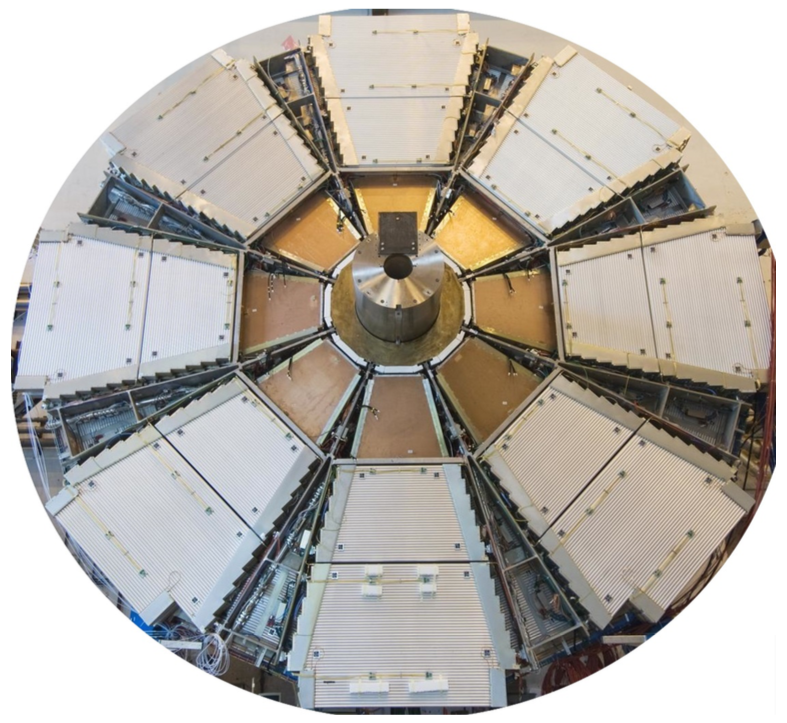
\includegraphics[width=0.48\textwidth]{figures/nsw/nsw_current_sw}
        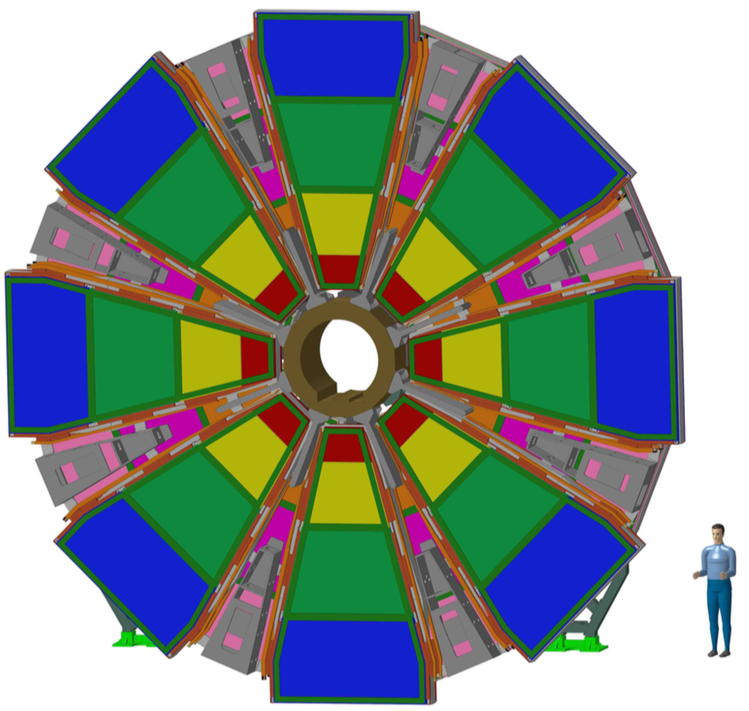
\includegraphics[width=0.48\textwidth]{figures/nsw/nsw_cartoon}
        \caption{
            \textit{Left}: Current Small Wheel detector (prior to installation in ATLAS), with CSC detectors (copper color) at low radii
                and MDT chambers (silver color) at higher radii.
            \textit{Right}: Geometry of the NSW, with a view of the large-sector side. The gaps in azimuth
                between the large sectors are instrumented with detectors on the side facing into the page.
        }
        \label{fig:nsw_geo}
    \end{center}
\end{figure}

\begin{figure}[!htb]
    \begin{center}
        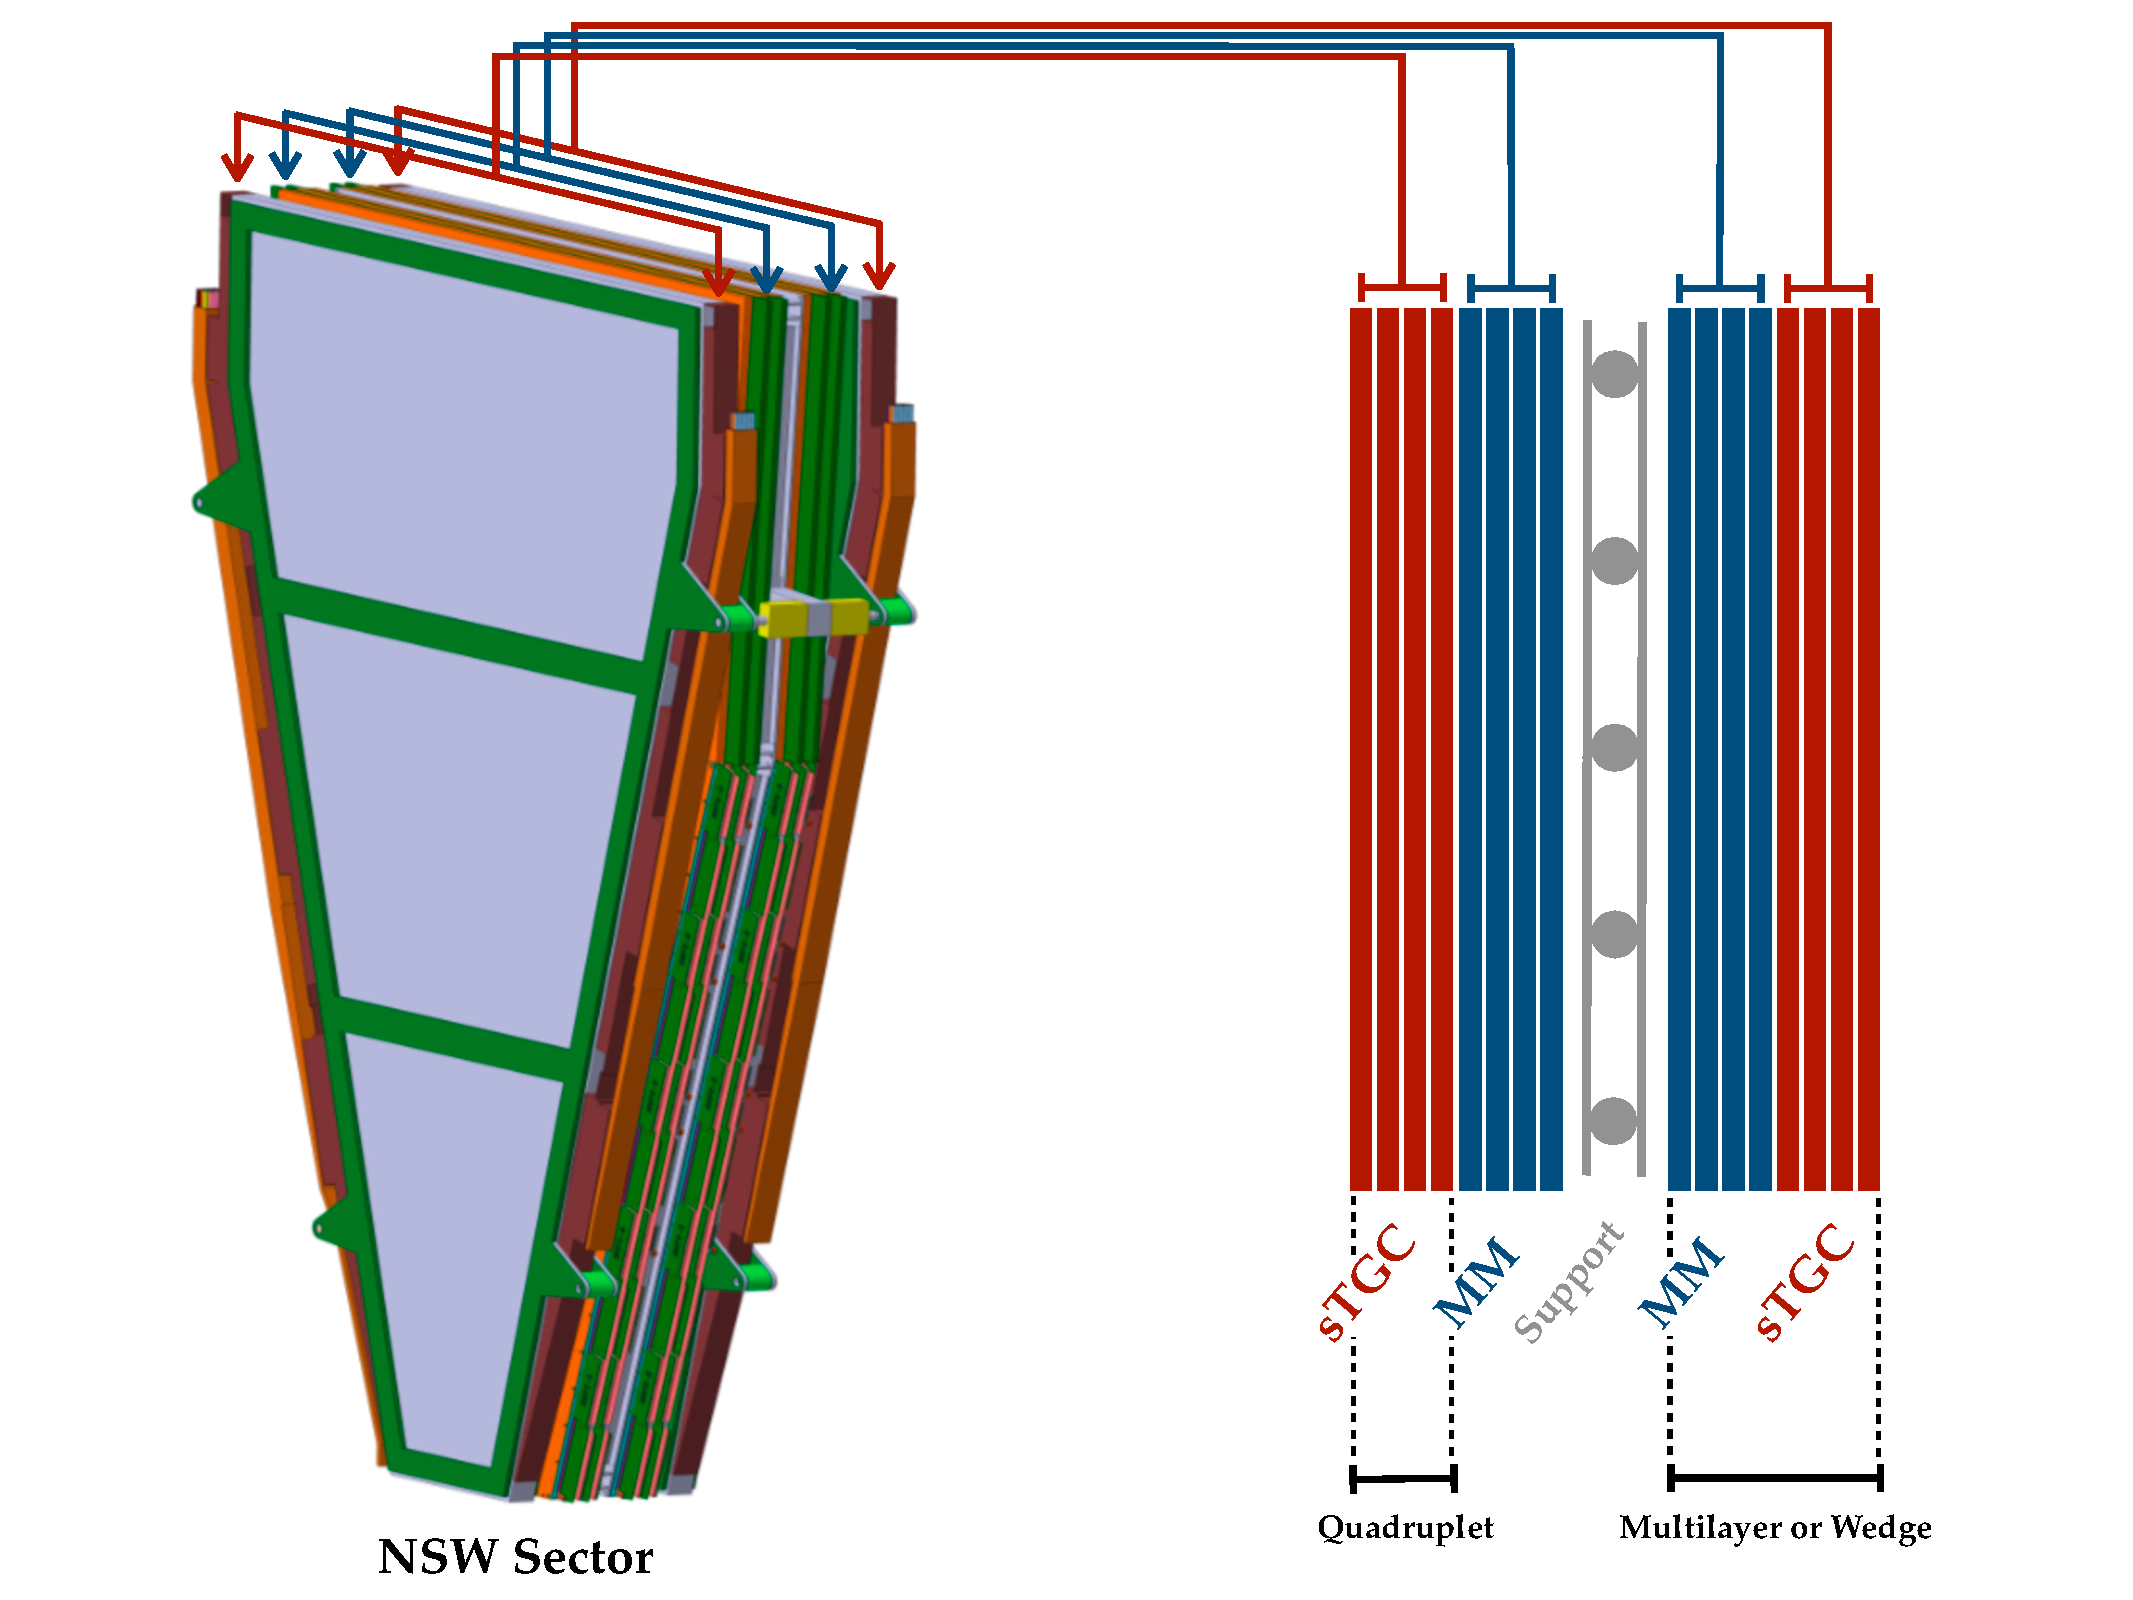
\includegraphics[width=0.8\textwidth]{figures/nsw/nsw_sector_layoutPDF}
        \caption{
            On the left is a mechanical drawing of an NSW sector, with the specific detector
            components illustrated on the right, composed of 16 detector planes: 8 MM layers
            sandwiched between 4 sTGC layers on either side.
            The base component of an NSW detector technology is a single detector plane,
            or layer, four of which are comprised in a single unit referred to as
            a `quadruplet'.
            A single side of the NSW, composed of an MM and sTGC quadruplet, is
            referred to as a `wedge' and a sector is referred to as a `double wedge'.
        }
        \label{fig:nsw_sector_layout}
    \end{center}
\end{figure}

%%%%%%%%%%%%%%%%%%%%%%%%%%%%%%%%%%%%%%%%%%%%%%%%%%%%%%%%%%%%%%%
% MICROMEGAS
%%%%%%%%%%%%%%%%%%%%%%%%%%%%%%%%%%%%%%%%%%%%%%%%%%%%%%%%%%%%%%%
\subsection{The Micromegas Detectors}
\label{sec:nsw_mm}

The MM detectors are designed with the high-precision tracking requirements of the HL-LHC
in mind, requiring a spatial precision better than $100\,\micron$.
They are characterised by readout strips with very fine segmentation and good
time resolution and can be exploited to complement the trigger scheme based on the sTGC, as
described above.

MM detectors are characterised by two asymmetric regions.
Standard MM detectors consist of a planar \textit{drift} electrode, a gas gap of
a few millimeters in thickness acting as a conversion and drift region, and a thin
metallic mesh at $\mathcal{O}(100)\,\micron$ above the readout electrodes.
The region between the mesh and readout electordes is the amplification region wherein
gain factors on the order of $10^4$ are achievable.

The electric potentials within the drift and avalanche regions are maintained
at a few hundred V/cm and $\approx50$\,kV/cm, respectively.
Charged particles traversing the drift space ionise the gas and the electrons, liberated
in the ionisation process, drift towards the mesh at timescales on the order of tens of nanoseconds.
The electron avalanche takes place in the amplification region in about a nanosecond,
resulting in a fast pulse on the readout electrode.

The MM detectors in the NSW are \textit{resistive-strip} MM detectors, characterised by an insulating
layer over the readout electrodes.
The insulating layer acts to protect the sensitive readout electrodes from sparking events that
reduce the detector performance over time.
Such sparking events ca cann happen frequently given the very large gas amplifications and high electric potentials
present in the amplification region.
Resistive strips on top of the insulating layer collect the avalanche electrons and induce
signals on copper readout strips embedded beneath the insulating layer.
Resistrive-strip MM detectors can sustain higher amplification and particle rates, a necessary
characteristic for targetting the high-luminosities foreseen at the HL-LHC.
The design and principle of operation of the resistive-strip MM technology is shown in Figure~\ref{fig:nsw_mm_principle},
in which incident MIPs traversing perpendicular and at an angle relative to the detector plane
are illustrated.

Each layer of an MM detector in the NSW is composed of $1023 \times 8$ readout strips, giving
a highly granular spatial readout allowing for high resolution position measurements to be made.
The MM quadruplets have two-dimensional readout, providing  both the $r$ ($\eta$)
and $\phi$ components of traversing particles.
%The two dimensional readout is achieved by tilting two of the readout planes in each of the
%MM quadruplets by $\pm 1.5$\,degrees to form a stereo readout. 
This is unlike the two-dimensional readout of the CSC detectors in the current Small Wheel detectors,
in which \textit{each} readout plane consists of perpendicular wires and strips providing
the two dimensional readout information.
This perpendicular readout, however, is susceptible to high rates of so-called \textit{ghost hits}
as a result of the geometrical ambiguities related to simultaneous hits across multiple readout elements, 
a common occurrence in high pileup conditions.
If the rates of these ghost hits are too high, the tracking performance of the detector will suffer non-negligibly.
In the case of perpendicular readout strips on the same readout plane, for example, there are $N_{\textit{ghost}} = (N^2 - N) \frac{p_1}{p_2}$
combinatorial ghost hits, where $N$ is the number of true hits, $p_1$, $p_2$ are the pitches\footnote{The readout strip pitch
is the inter-strip distance of the readout plane of the detector.} of the first and
second detector plane responsible for the readout of the first and second coordinates, respectively.
In the NSW, $p_1 = p_2 = \mathcal{O}(100)\,\micron$.
The combinatorial ambiguities are resolved by tilting the readout planes at angles relative to
each other.
The principle of the stereo readout and its implementation within the MM quadruplets in the NSW
is illustrated in Figure~\ref{fig:mm_stereo}.
The tilt angle used for the NSW MM detectors is $\pm 1.5$\,degrees and has been optimised so as to simultaneously minimise
the number of ghost hits and the spatial reconstruction in the $r$ and $\phi$ directions.
The stereo-angle two-dimensional readout contributes to the ability of the MM detectors' ability
to maintain high-precision tracking performance even in the highest rates foreseen for the HL-LHC.

\begin{figure}[!htb]
    \begin{center}
        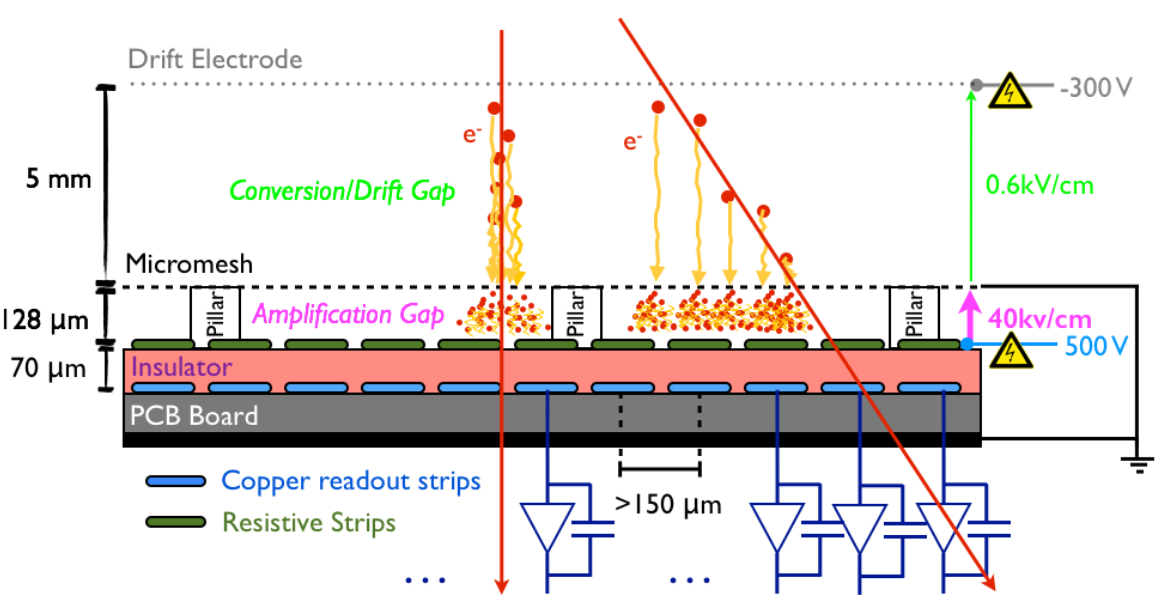
\includegraphics[width=0.8\textwidth]{figures/nsw/nsw_mm_principle}
        \caption{
        }
        \label{fig:nsw_mm_principle}
    \end{center}
\end{figure}

\begin{figure}[!htb]
    \begin{center}
        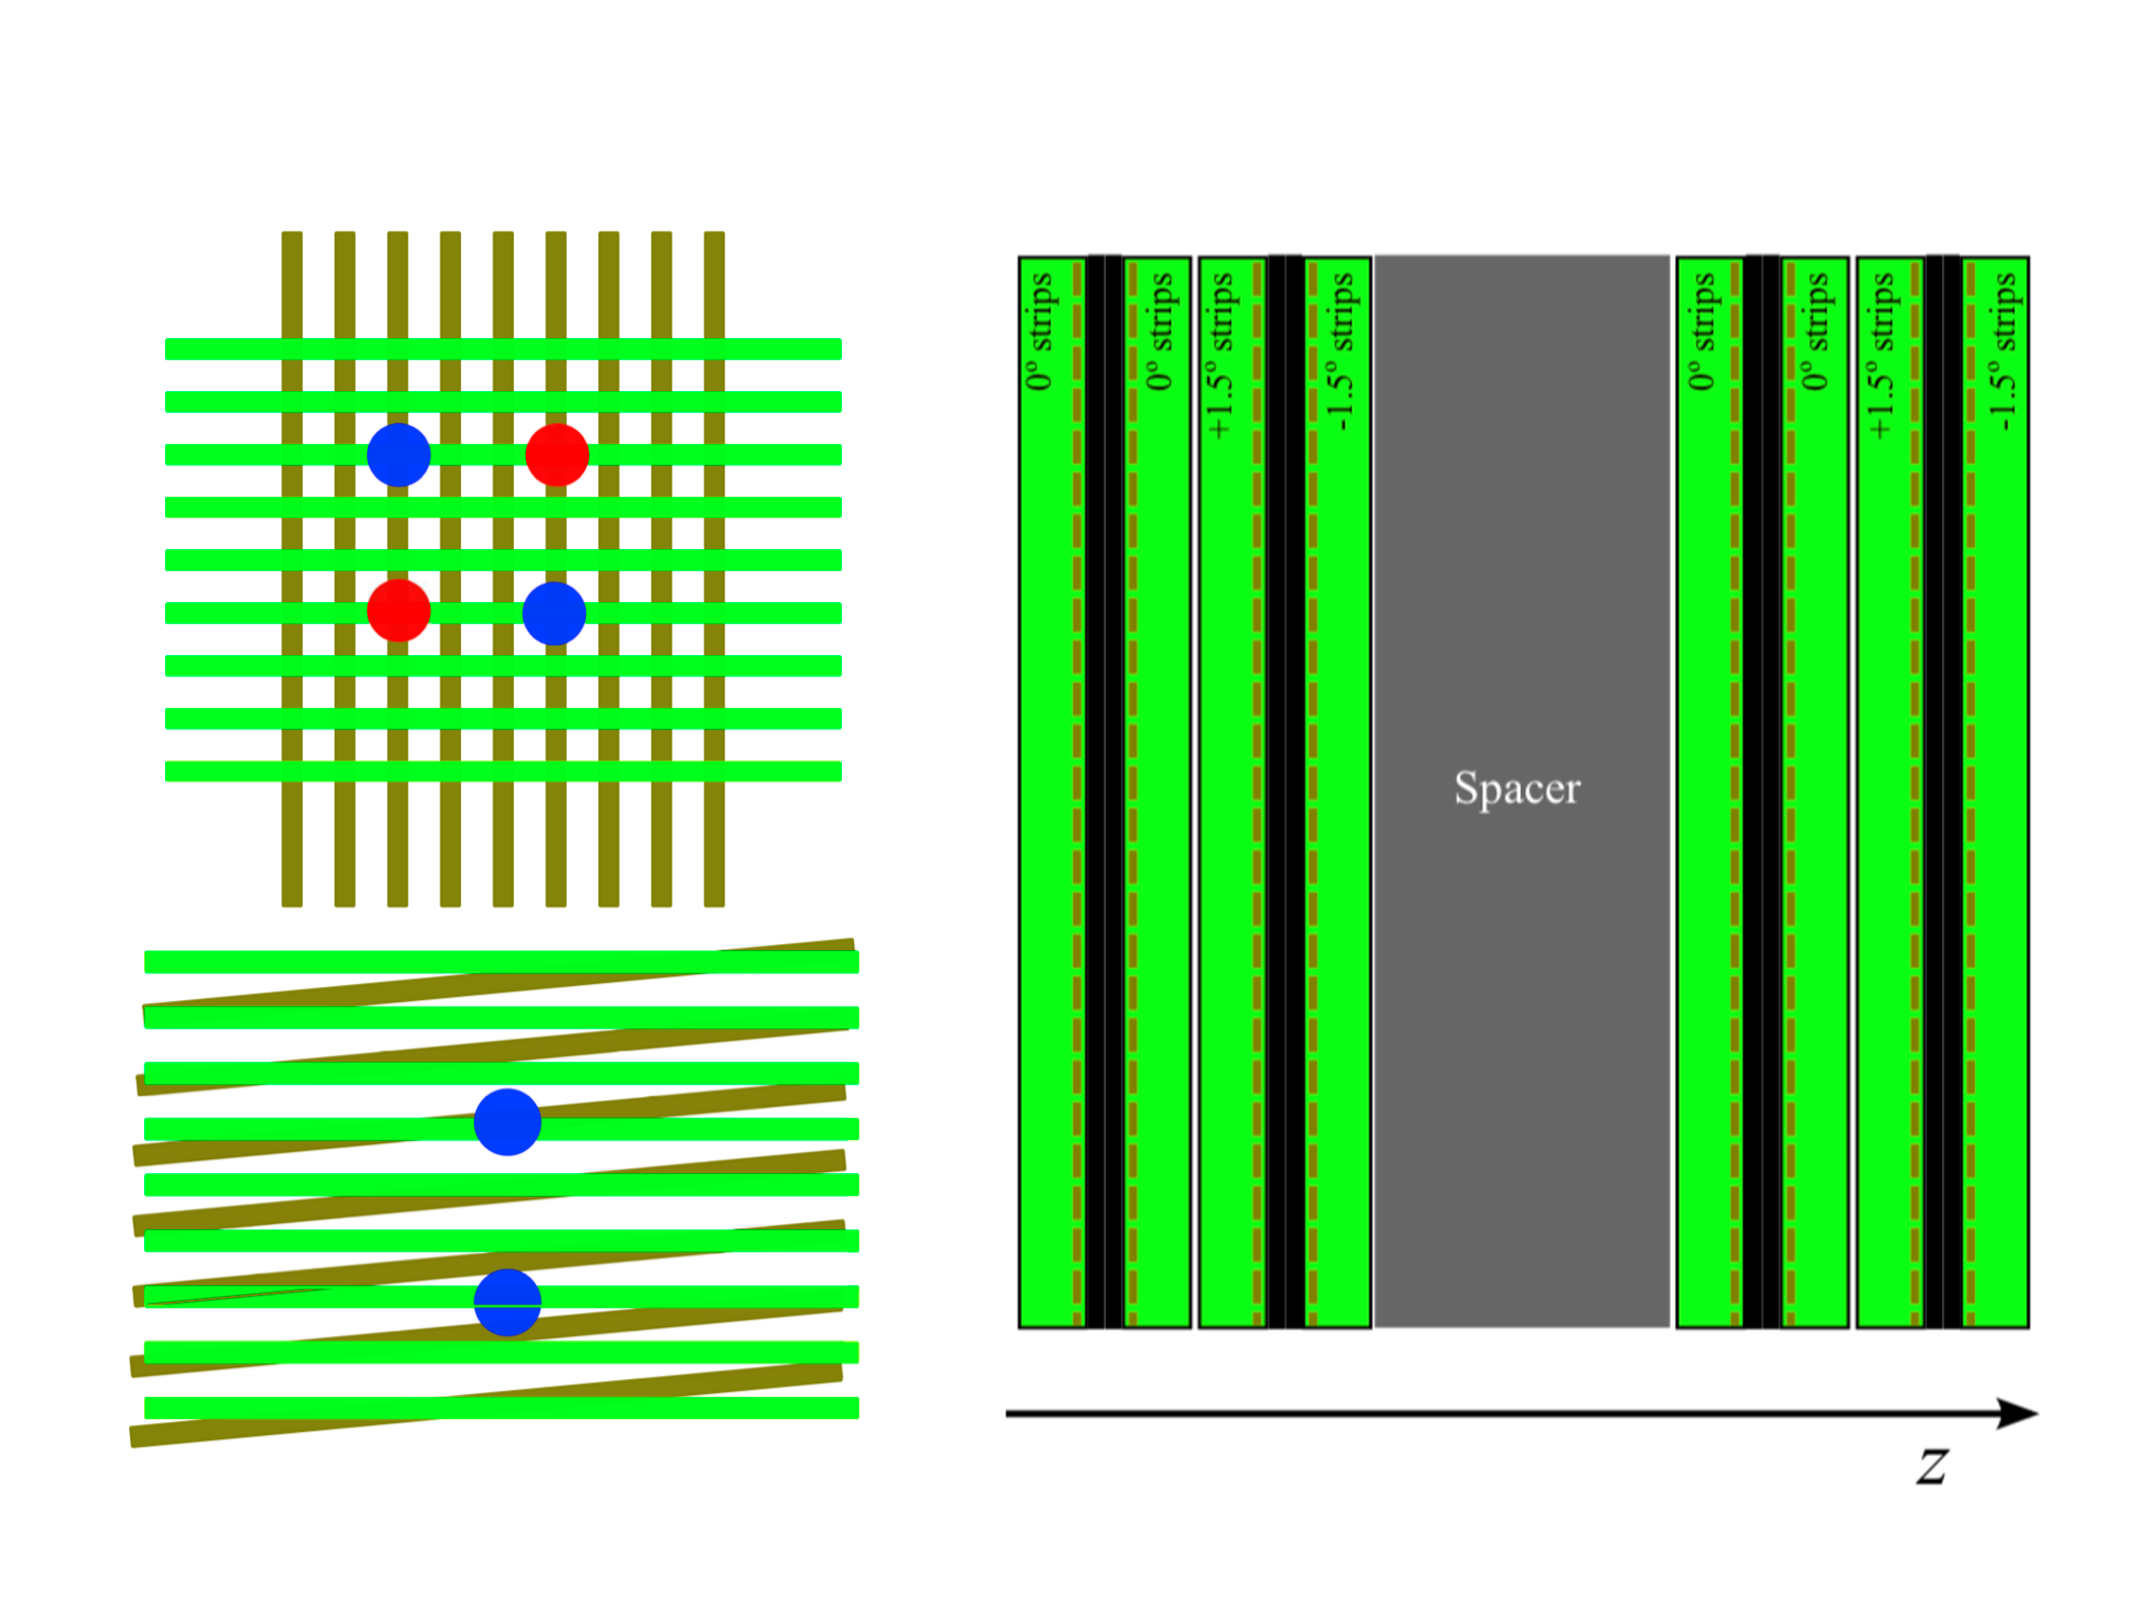
\includegraphics[width=0.8\textwidth]{figures/nsw/mm_ghost_stereoPDF}
        \caption{
        }
        \label{fig:mm_stereo}
    \end{center}
\end{figure}

%%%%%%%%%%%%%%%%%%%%%%%%%%%%%%%%%%%%%%%%%%%%%%%%%%%%%%%%%%%%%%%
% STGC
%%%%%%%%%%%%%%%%%%%%%%%%%%%%%%%%%%%%%%%%%%%%%%%%%%%%%%%%%%%%%%%
\subsection{The Small-strip Thin Gap Chamber Detectors}
\label{sec:nsw_stgc}
